%%%%%%%%%%%%%%%%%%%%%%%%%%%%%%%%%%%%%%%%%%%%%%%%%%%%%%%%%%%%%%%%%%%%%%%%%%%%%
%% Original default rstudio/pandoc latex file
%% upated by @jhollist 09/15/2014
%% inspired by @cboetting https://github.com/cboettig/template and
%% @rmflight blog posts:
%% http://rmflight.github.io/posts/2014/07/analyses_as_packages.html 
%% http://rmflight.github.io/posts/2014/07/vignetteAnalysis.html).  
%%%%%%%%%%%%%%%%%%%%%%%%%%%%%%%%%%%%%%%%%%%%%%%%%%%%%%%%%%%%%%%%%%%%%%%%%%%%%

\documentclass[11pt,a4paper]{article}
\usepackage[T1]{fontenc}
\usepackage{lmodern}
\usepackage{amssymb,amsmath}
\usepackage{ifxetex,ifluatex}
\usepackage{fixltx2e} % provides \textsubscript
% use upquote if available, for straight quotes in verbatim environments
\IfFileExists{upquote.sty}{\usepackage{upquote}}{}
\ifnum 0\ifxetex 1\fi\ifluatex 1\fi=0 % if pdftex
  \usepackage[utf8]{inputenc}
\else % if luatex or xelatex
  \ifxetex
    \usepackage{mathspec}
    \usepackage{xltxtra,xunicode}
  \else
    \usepackage{fontspec}
  \fi
  \defaultfontfeatures{Mapping=tex-text,Scale=MatchLowercase}
  \newcommand{\euro}{€}
\fi
% use microtype if available
\IfFileExists{microtype.sty}{\usepackage{microtype}}{}
\usepackage[margin=1in]{geometry}
\ifxetex
  \usepackage[setpagesize=false, % page size defined by xetex
              unicode=false, % unicode breaks when used with xetex
              xetex]{hyperref}
\else
  \usepackage[unicode=true]{hyperref}
\fi
\hypersetup{breaklinks=true,
            bookmarks=true,
            pdfauthor={},
            pdftitle={Agreement Attraction in Turkish: Effects of Nominal and Verbal Plural Morphemes},
            colorlinks=true,
            citecolor=blue,
            urlcolor=blue,
            linkcolor=magenta,
            pdfborder={0 0 0}}
\urlstyle{same}  % don't use monospace font for urls
\setlength{\parindent}{0pt}
\setlength{\parskip}{6pt plus 2pt minus 1pt}
\setlength{\emergencystretch}{3em}  % prevent overfull lines
\setcounter{secnumdepth}{5}

%%%%%%%%%%%%%%%%%%%%%%%%%%%%%%%%%%%%%%%%%%%%%%%%%%%%%%%%
%Changes borrowed from @cboettig, added by @jhollist 
% A modified page layout 
\textwidth 6.75in
\oddsidemargin -0.15in
\evensidemargin -0.15in
\textheight 9in
\topmargin -0.5in
\usepackage{lineno} % add 
  \linenumbers % turns line numbering on 
%%%%%%%%%%%%%%%%%%%%%%%%%%%%%%%%%%%%%%%%%%%%%%%%%%%%%%%%

%%%%%%%%%%%%%%%%%%%%%%%%%%%%%%%%%%%%%%%%%%%%%%%%%%%%%%%%
%%Packages and layout changes by @jhollist 09/15/2014
\usepackage{ragged2e}
\usepackage[font=normalsize]{caption}
  \usepackage[singlespacing]{setspace}
\usepackage{parskip}
\usepackage{fancyhdr}
\pagestyle{fancy}
\fancyhf{}
\renewcommand{\headrulewidth}{0pt}
  \rfoot{\today}
\lfoot{\thepage}
%%Changed default abstract width and added lines
\renewenvironment{abstract}{
  \hfill\begin{minipage}{1\textwidth}
  \rule{\textwidth}{1pt}\vspace{5pt}
  \normalsize
  \begin{justify}
  \bfseries\abstractname\vspace{5pt}
  \end{justify}}
  {\par\noindent\rule{\textwidth}{1pt}\end{minipage}
}
%%%%%%%%%%%%%%%%%%%%%%%%%%%%%%%%%%%%%%%%%%%%%%%%%%%%%%%%

\title{Agreement Attraction in Turkish: Effects of Nominal and Verbal Plural
Morphemes}
\author{
Utku Turk
Pavel Logacev
}
\date{}
% Allowing for landscape pages
\usepackage{lscape}
\newcommand{\blandscape}{\begin{landscape}}
\newcommand{\elandscape}{\end{landscape}}

% Left justification of the text: see https://www.sharelatex.com/learn/Text_alignment
% \usepackage[document]{ragged2e} % already in the latex template
\newcommand{\bleft}{\begin{flushleft}}
\newcommand{\eleft}{\end{flushleft}}

% multicols
\usepackage{multicol}
\usepackage{paracol}

% enumerated examples
\usepackage{enumitem}

% for linguistic examples &  interlinear glosses
\usepackage{gb4e}
\exewidth{(10.159)}
\noautomath
\let\eachwordone=\it

\usepackage{qtree}	


% for figure and table side by side
\usepackage{floatrow}
\newfloatcommand{btabbox}{table}

%%Fix tightlist error: https://stackoverflow.com/questions/40438037/tightlist-error-using-pandoc-with-markdown
%%Added 2018-03-26 
\providecommand{\tightlist}{%
  \setlength{\itemsep}{0pt}\setlength{\parskip}{0pt}}
%%%  
  

\begin{document}
%%Edited by @jhollist 09/15/2014
%%Adds title from YAML
\begin{singlespace}
\begin{center}
\huge Agreement Attraction in Turkish: Effects of Nominal and Verbal Plural
Morphemes
\end{center}
%%Adds Author, correspond email asterisk, and affilnum from YAML
\begin{center}
\large
Utku Turk \textsuperscript{*} \textsuperscript{1} 
Pavel Logacev \textsuperscript{1} 
\end{center}
%%Adds affiliations from YAML
\begin{justify}
\footnotesize \emph{ 
\\*
\textsuperscript{1}Bogazici University, South Campus, John Freely Building, Department of
Linguistics, 34342, Istanbul, Turkey\\*
}
%%Adds corresponding author email(s) from YAML
\newcounter{num}
\setcounter{num}{1}
\\[0.1cm]
\footnotesize \emph{ 
\ifnum\value{num}=1%
\textsuperscript{*} corresponding author:
\fi
\href{mailto:utku.turk@boun.edu.tr}{\nolinkurl{utku.turk@boun.edu.tr}}
\stepcounter{num}
}
\end{justify}
%%Adds date from YAML
\normalsize

\end{singlespace}


\vspace{2mm}\hrule

In this paper, our objective is to explore the source of agreement
attraction effects in Turkish discovered by Lago (2018). The
interpretation of their finding is complicated by the fact that the
possessive form of all head nouns used in their stimuli are
morphologically ambiguous between possessive and accusative. In Turkish,
genitive can be productively used for marking the subject of an embedded
clause whereas accusative is rarely used for marking the subject. Due to
this mismatch in the frequency of usage of accusative and genitive,
which is used as a attractor in this experiment, as a controller, Lago
(2018)'s findings could potentially be explained with occasional shallow
processing. We have replicated Lago (2018)'s experiment with unambigious
head nouns, and we have found similar agreement attraction effects.
However, this may mean that participants engage in even more shallow
processing than we imagined. We postulate that participants solely check
for the presence of a \emph{-lAr} morpheme, while largely disregarding
the remainder of the sentence. We utilize an experiment design in which
we use a relative clause with or without plural agreement on the verb in
place of the genitive possessor since both verbal and nominal plural
morphemes are the same in Turkish, i.e.~the exponent of both is
\emph{-lAr}. If participants did, in fact, adopt a superficial
processing strategy, we would expect to find a number agreement
attraction effect similar in magnitude to that in Lago (2018). However,
if number attraction is not an artifact of shallow processing
strategies, we should expect to find no number attraction effects in
this experiment.

\vspace{3mm}\hrule

\emph{Keywords}: Turkish, agreement attraction, task effect, shallow
processing

\bleft

\hypertarget{introduction}{%
\section{INTRODUCTION}\label{introduction}}

Attraction errors in the production and comprehension of subject-verb
agreement, in which a verb does not agree with the grammatical agreement
controller, but with a potential attractor, have been the main topic of
research in many studies for quite a long time. In fact, it is still a
widely researched area in psycholinguistic studies. Despite the
comprehensive research that has been carried out, studies that have been
conducted on agreement attraction in Turkish have been very limited. In
fact, Lago (2018) is currently the only study that explores this
phenomenon in Turkish. Lago (2018) makes use of genitive-possessive
structures in the subject position, in which the possessive-marked noun
is the head of the noun phrase which acts as the grammatical agreement
controller, and the genitive noun serves as a potential attractor. In a
speeded acceptability judgment study, Lago (2018) found a significant
effect of number agreement attraction. However, the interpretation of
their findings may be a result of the fact that non-subjecthood cues
originate from their use of morphologically ambiguous forms of the
possessive. In the possessive forms that are used, all the head nouns in
their stimuli are ambigiuous between possessive and accusative.

In Turkish, accusative number agreement controllers are extremely rare,
while genitive agreement controllers are very frequent. Thus, Lago
(2018)'s finding could potentially be explained with occasional shallow
processing. When all syntactic relations in the sentence were processed
fully, the possessive noun may have been identified as the controller.
Meanwhile, the genitive noun may sometimes have been erroneously
identified as the controller during shallow processing because genitives
are more likely to act as agreement controllers than accusatives
(SOURCE). A second alternative explanation for Lago (2018)'s findings
may be the fact that participants may engage in even more shallow
processing than outlined above. Participants may have erroneously
responded \emph{Yes} on some trials for two main reasons: (i) the
presence of a plural morpheme on a noun (attractor or controller), and
(ii) the presence of a plural agreement morpheme on the verb. We
speculate that in such trials, participants would have simply tried to
check for the presence of such morphemes, while largely disregarding the
remainder of the sentence.

We first replicated Lago (2018)'s experiment with unambiguous head
nouns. To this end, we revised the items that were used previously in
order to avoid morphological ambiguity between possessive and accusative
forms. The effect found in Lago (2018) was also observed when
unambiguous nouns were used, as will be discussed in \S 2.

\S 3 discusses the alternative account that posits even more shallow
processing as mentioned above and presents a pre-registered experiment
using RC attractors with potential outcomes and their indications. Since
both nominal and verbal plural morphemes in Turkish are expressed with
the same form (\emph{-ler} or \emph{-lar} depending on the phonological
environment), we can test this possibility with an experiment in which a
relative clause with or without plural agreement on the verb in place of
the genitive possessors is used. An agreement attraction effect similar
in magnitude to that observed in Lago (2018) would indicate that
participants use the aforementioned strategies.

\S 4 offers a discussion of the issue of number attraction and where
this experiments leaves us. Lastly, \S 5 presents a brief conclusion and
topics for future research.

\hypertarget{replicaton-of-lago-et-al.-2018}{%
\section{REPLICATON OF LAGO ET AL.
(2018)}\label{replicaton-of-lago-et-al.-2018}}

In their study, Lago (2018) investigate the comprehension of
subject-verb agreement in Turkish-German bilinguals and Turkish
monolinguals. They use speeded acceptability judgments for the effects
of number attraction in Turkish. Their sentences make us of
genitive-possessive constructions in the subject position, where the
genitive is the attractor and the possessive is the head noun. They
manipulate the grammaticality of the sentence by changing the plural
morphology of the verb, and they also manipulate the plurality of the
attractor noun. In grammatical conditions, the subject and the verb both
bear singular morphology with no overt morpheme. Moreover, in the
ungrammatical conditions, the verb bears the overt \emph{-lAr} morpheme
whereas the subject is still singular as exemplified below.

\begin{exe}
\ex
\begin{xlist}
\ex \underline{Grammatical, SG attractor} \label{lago1}
\gll \c{S}ark{\i}c{\i}-n{\i}n vokalist-i sahne-de s\"{u}rekli z{\i}pla-d{\i}\\
singer-\textsc{gen} vocalist-\textsc{poss} stage-\textsc{loc} non-stop jump-\textsc{pst}-$\varnothing$\\
\glt The singer's backup vocalist jumped on the stage non-stop.

\ex \underline{Grammatical, PL attractor} \label{lago2}
\gll \c{S}ark{\i}c{\i}-lar-{\i}n vokalist-i sahne-de s\"{u}rekli z{\i}pla-d{\i}\\
singer-\textsc{pl}-\textsc{gen} vocalist-\textsc{poss} stage-\textsc{loc} non-stop jump-\textsc{pst}-$\varnothing$\\
\glt The singers' backup vocalist jumped on the stage non-stop.

\ex \underline{Ungrammatical, PL attractor} \label{lago3}
\gll \c{S}ark{\i}c{\i}-lar-{\i}n vokalist-i sahne-de s\"{u}rekli z{\i}pla-d{\i}-lar.\\
singer-\textsc{pl}-\textsc{gen} vocalist-\textsc{poss} stage-\textsc{loc} non-stop jump-\textsc{pst}-\textsc{3Pl}\\
\glt The singers' backup vocalist jumped on the stage non-stop.

\ex \underline{Ungrammatical, SG attractor} \label{lago4}
\gll \c{S}ark{\i}c{\i}-n{\i}n vokalist-i sahne-de s\"{u}rekli z{\i}pla-d{\i}-lar.\\
singer-\textsc{gen} vocalist-\textsc{poss} stage-\textsc{loc} non-stop jump-\textsc{pst}-\textsc{3Pl}\\
\glt The singer's backup vocalist jumped on the stage non-stop.
\end{xlist}
\end{exe}

They found a significant effect of number attraction in Turkish ranging
between 11\%--15\% across monolinguals. As seen in the results of the
statistical analysis in \textsc{Table} (\ref{lagomodel}), the
acceptability judgments showed an immense effect of grammaticality, and
there is also interaction between grammaticality and attractor number,
which indicates the presence of a number attraction effect.

\begin{table}[!hbt]
\centering
\begin{tabular}{llcccc}
\hline
    &                                        & \multicolumn{4}{l}{Monolingual Speakers}                                               \\ \cline{3-6} 
    &                                        & $\beta$        & SE            & \emph{z} & \emph{p} \\ \hline
\multicolumn{2}{l}{\textbf{Attraction Task}} &                &               &                           &                           \\
    & Grammaticality                         & \textbf{-5.51} & \textbf{0.33} & \textbf{-16.69}           & \textbf{.000}             \\
    & Attractor Number                       & 0.14           & 0.25          & 0.57                      & .571                      \\
    & Grammaticality x Attractor Number      & \textbf{1.69}  & \textbf{0.53} & \textbf{3.19}             & \textbf{.001}             \\
    & Attractor Number: Ungram conditions    & \textbf{0.94}  & \textbf{0.26} & \textbf{3.68}             & \textbf{.000}             \\
    & Attractor Number: Gram conditions      & -0.79          & 0.52          & -1.51                     & .131                      \\ \hline
\end{tabular}
\caption{Model results for the judgments of monolingual cited from @Lago.}
\label{lagomodel}
\end{table}

Lago (2018) stipulate that the Turkish genitive case does not provide a
strong cue against subjecthood since Turkish frequently makes use of
genitive marked subjects in embedded clauses, as in example
(\ref{gensubj}). This is in contrast with English, in which the genitive
case is compatible with subjecthood. Thus, Lago (2018) argue that this
robust agreement attraction effect has been linked to the case
information carried by accusative and genitive.

\begin{exe}
\ex \label{gensubj}
\gll k\"{o}y-\"{u} bir haydut-un bas-t{\i}\u{g}-{\i}n-{\i} duy-du-m.\\
village-\textsc{acc} a bandit-\textsc{gen} raid-\textsc{nmlz}-\textsc{3Sg}-\textsc{acc} hear-\textsc{pst}-\textsc{1Sg}\\
\glt I heard that a (certain) robber raided the village. (Adapted from Woolford (2009))
\end{exe}

However, our initial hypothesis postulates that participants engage in
shallow processing, which results in a situation in which not only the
genitive case but also the possessive case plays a significant role in
delivering the case information. None of the experimental items in Lago
(2018) have a head noun which ends with a vowel; thus, all of the
possessive markers are morphologically and phonologically ambiguous
between the accusative case and the possessive. Unlike genitive case, it
is extremely rare for the accusative case to appear on the head noun of
the subject, which only occurs in raising predicates as in example
(\ref{dsm}).

\begin{exe}
\ex \label{dsm}
\gll Ben sen-i git-ti-n san-d{\i}-m\\
I you-\textsc{acc} go-\textsc{pst}-\textsc{2Sg} suppose-\textsc{pst}-\textsc{1Sg}\\
\glt I thought you were gone.
\end{exe}

In order to test this hypothesis, we have replicated the experiment of
Lago (2018) with modified items, in which the possessive is not
ambiguous with the accusative case. We tried to be as faithful as
possible to the original sentences while also trying to make the
sentences as plausable as possible. We keep the semantic relation
between the head noun and the controller the same with what has been
described in Lago (2018)'s study, which is either a relation regarding
profession or a service that is given by the head noun for the
possessor. A set of sentences are exemplified below.

\begin{exe}
\ex
\begin{xlist}
\ex \underline{Grammatical, SG attractor} \label{exp1}
\gll Komedyen-in yard{\i}mc{\i}-s{\i} poyraz-dan dolayi \"{u}\c{s}\"{u}-d\"{u}.\\
comedian-\textsc{gen} helper-\textsc{poss} northeaster-\textsc{abl} because.of feel.chilly-\textsc{pst}-$\varnothing$\\
\glt Because of the northeaster, comedian's assistant felt chilly.

\ex \underline{Grammatical, PL attractor} \label{exp2}
\gll Komedyen-ler-in yard{\i}mc{\i}-s{\i} poyraz-dan dolayi \"{u}\c{s}\"{u}-d\"{u}.\\
comedian-\textsc{pl}-\textsc{gen} helper-\textsc{poss} northeaster-\textsc{abl} because.of feel.chilly-\textsc{pst}-$\varnothing$\\
\glt Because of the northeaster, comedians' assistant felt chilly.

\ex \underline{Ungrammatical, PL attractor} \label{exp3}
\gll Komedyen-ler-in yard{\i}mc{\i}-s{\i} poyraz-dan dolayi \"{u}\c{s}\"{u}-d\"{u}-ler.\\
comedian-\textsc{pl}-\textsc{gen} helper-\textsc{poss} northeaster-\textsc{abl} because.of feel.chilly-\textsc{pst}--\textsc{pl}\\
\glt Because of the northeaster, comedians' assistant felt chilly.

\ex \underline{Ungrammatical, SG attractor} \label{exp4}
\gll Komedyen-in yard{\i}mc{\i}-s{\i} poyraz-dan dolayi \"{u}\c{s}\"{u}-d\"{u}-ler.\\
comedian-\textsc{gen} helper-\textsc{poss} northeaster-\textsc{abl} because.of feel.chilly-\textsc{pst}-\textsc{pl}\\
\glt Because of the northeaster, comedian's assistant felt chilly.

\end{xlist}
\end{exe}

As seen in the examples, unlike Lago (2018)'s experimental items, all of
our items bear the \emph{-sI} possessive marker instead of the ambiguous
\emph{-I} marker. As for the filler items, we could not use or modify
the original experiment items since the fillers of the original study
were not online. We have used two types filler sentences: grammatical
sentences in which the verb bears plural agreement (\ref{fillera}), and
ungrammatical sentences in which the verb does not bear plural agreement
(\ref{fillerb}). We wanted to nullify a possible strategy by the
participants where they associate the sentence-final morpheme directly
with the acceptability of the sentence. And we also wanted to eliminate
the possibility of participants disregarding other elements in the
sentences while answering the questions we ask right after the sentence.

\begin{exe}
\ex
\begin{xlist}
\ex \label{fillera}
\gll Adam-{\i}n anne-si fena-la\c{s}-{\i}nca inek kurban et-ti-ler.\\
man-\textsc{gen} mother-\textsc{poss} bad-\textsc{vrb}-\textsc{cvb} cow sacrifice do-\textsc{pst}-\textsc{pl}\\
\glt When his mother got ill, (they) sacrificed a cow.
\ex \label{fillerb}
\gll *Pizzac{\i}-n{\i}n kurye-si t\"{o}kezle-yince sos-lar yer-e sa\c{c}-t{\i}.\\
pizzaria-\textsc{gen} courier-\textsc{poss} trip-\textsc{cvb} sauce-\textsc{pl} floor-\textsc{dat} scatter-\textsc{pst}\\
\glt Intended: When the pizza boy tripped, sauces scattered around. 
\end{xlist}
\end{exe}

All of our data, experimental materials, our experiment design, and our
fillers can be found on the website of the Center for Open Science
Framework (\url{https://osf.io/}).

\hypertarget{participants-and-procedure}{%
\subsection{Participants and
Procedure}\label{participants-and-procedure}}

One hundred and seven Turkish speakers with a mean age of X were
recruited from Bogazici University in İstanbul. We did not collect
participants' knowledge of other languages; however, we verified that
Turkish is their native language and that they predominantly use it in
their daily lives. In the experiments, participants were asked to judge
the acceptability of experimental and filler sentences in Turkish. All
of the sentences were presented one word at a time in the center of the
screen for 500 ms per word unlike Lago (2018) and Wagers et al. (2009),
in which the duration was 300 ms per word. The experiment was run on a
web-based platform titled the Ibex Farm, and all of the documentation
can be found on our osf and github page.

Before the experiment, participants were instructed to give accurate and
quick answers based on their own intuitions, and they were also notified
about the time limit for answering. At the start of the experiment, they
were given 4 practice items with feedback.

What to write about analyze?

\hypertarget{results-and-discussion}{%
\subsection{Results and Discussion}\label{results-and-discussion}}

In \textsc{Figure} (1), the y-axis shows the percentage of
``acceptable'' answers, and the x-axis indicates whether or not the
sentences in that group are grammatical. Moreover, the linet ypes
indicate an attractor noun with overt plural morphology. As seen in the
figure, 22\% of the sentences with plural attractors and a singular verb
were accepted by the participants, in line with the findings of Lago
(2018). We also see a number attraction rate of 10\% which was also
observed in Lago (2018) with close results.

In \textsc{Table} (\ref{tab:replication}),
\ldots{}\ldots{}\ldots{}\ldots{}

And yes, I plan to beautify the figures.

\begin{figure}[H]
  \begin{floatrow}
    \ffigbox{%

\begin{flushright}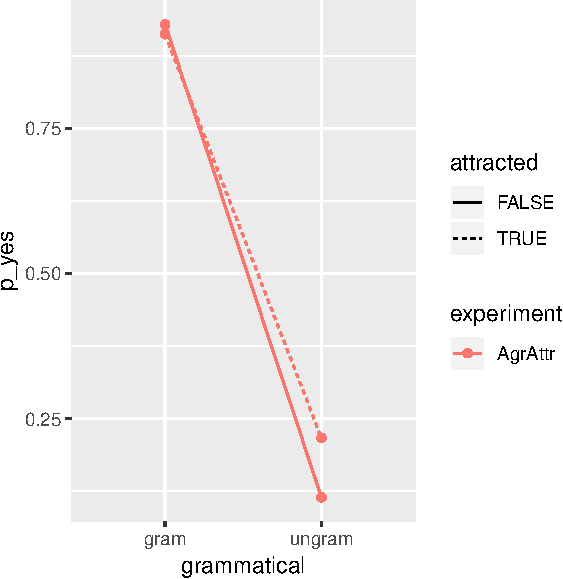
\includegraphics{output/figures/unnamed-chunk-1-1} \end{flushright}
    }{\caption{A figure}}

    \btabbox{%

    }{\caption{A table}}
  \end{floatrow}
\end{figure}

\hypertarget{experiment-2-rc-attractor}{%
\section{EXPERIMENT 2: RC ATTRACTOR}\label{experiment-2-rc-attractor}}

Even though our first hypothesis regarding shallow processing did not
hold, we still need to entertain the second possibility we have
discussed in this paper. Participants may indeed engage in an even
shallower process of sentence comprehension, in which they merely match
the use of \emph{-lAr}. Moreover, we still need to discuss how much it
is an effect of case information rather than only a number attraction.
We have seen that the anti-subjecthood cues of the accusative are not
significant since in both cases where the possessive is ambiguous with
the accusative and the possessive is clearly marked, we have observed
extremely close results in the speeded acceptability judgments.

In order to check both the sole effect of number agreement and the
possibility of a task effect, we propose an experiment design in which a
head noun is a bare NP, is not marked with any other morpheme and
preceded by a relative clause construction. This relative clause
consists of only a verbal component, which bears an overt plural marker.
Since Turkish verbal and nominal plural morphemes are identical, we plan
to check the participants' strategy with regards to whether or not it is
a cue that helps in the reconstruction of the ungrammatical sentence or
whether it is merely a task effect in which participants disregard the
rest of the sentence and focus the existence of the morpheme
\emph{-lAr}.

\hypertarget{materials}{%
\subsection{Materials}\label{materials}}

Like genitive-possessive structures, attractors do not intervene between
the grammatical agreement controller and the verb in relative clause
constructions. Turkish relative clauses always precede the head noun,
except for in special cases in which they are marked with unique
prosody. Item (\ref{rcexample}) is an example of a RC structure, and
item (\ref{rcexample2}) shows the possibility of using only the verbal
component of the relative clause since it is grammatical to drop
arguments in Turkish. ( add a footnote here giving the details of such
events, and restrictions. )

\begin{exe}
\ex
\begin{xlist}
\ex \label{rcexample}
\gll On-lar-{\i}n ev-e gel-me-den g\"{o}r-d\"{u}k-ler-i \c{c}ocuk so\u{g}uk-ta \"{u}\c{s}\"{u}-m\"{u}\c{s}-t\"{u}.\\
they-\textsc{pl}-\textsc{gen} home-\textsc{dat} come-\textsc{neg}-\textsc{abl} see-\textsc{nlmz}-\textsc{pl}-\textsc{poss} kid cold--\textsc{loc} feel.chilly-\textsc{perf}-\textsc{pst}\\
\glt The kid that they saw right before coming to home was feeling chilly. 
\ex \label{rcexample2}
\gll G\"{o}r-d\"{u}k-ler-i \c{c}ocuk so\u{g}uk-ta \"{u}\c{s}\"{u}-m\"{u}\c{s}-t\"{u}.\\
see-\textsc{nlmz}-\textsc{pl}-\textsc{poss} kid cold--\textsc{loc} feel.chilly-\textsc{perf}-\textsc{pst}\\
\glt The kid that they saw home was feeling chilly.
\end{xlist}
\end{exe}

As for the experimental sentences, we plan to use sentences that are
similar to the ones used in Lago (2018). Instead of a genitive
controller, we utilize an RC, which we manipulate for its values for
bearing the plural morpheme. The head noun of the subject is always
singular, and it is followed by a 2/3 word adverbial. Moreover, the
matrix verb of the sentences is also manipulated in terms of plurality,
deeming the sentence grammatical or ungrammatical. Lastly, the relative
clause has to be an object relative clause, since Turkish subject
relative clauses never bear a plural morpheme on the embedded verb. As
in the Lago (2018)'s study and our replication, we will have a four
condition, where we manipulate the plurality of the attractor
(\emph{plural/singular}) and the grammaticality of the sentece by using
overt plural morphology (\emph{grammatical/ungrammatical}), which are
demonstrated with item (\ref{reg1}), (\ref{reg2}), (\ref{reg3}), and
(\ref{reg4})

\begin{exe}
\ex
\begin{xlist}
\ex \underline{Grammatical, SG attractor} \label{reg1}
\gll D\"{o}v-d\"{u}\u{g}-\"{u} \c{c}ocuk mutfak-ta bayg{\i}n hal-de yat-{\i}yor-du.\\
beat-\textsc{nmlz}-\textsc{poss} kid kitchen-\textsc{loc} unconscious state-\textsc{loc} lie-\textsc{prog}-\textsc{pst}\\ 
\glt The kid that he/she beats was laying in the kitchen unconscious.
\ex \underline{Grammatical, PL attractor} \label{reg2}
\gll D\"{o}v-d\"{u}k-ler-i \c{c}ocuk mutfak-ta bayg{\i}n hal-de yat-{\i}yor-du.\\
beat-\textsc{nmlz}-\textsc{pl}-\textsc{poss} kid kitchen-\textsc{loc} unconscious state-\textsc{loc} lie-\textsc{prog}-\textsc{pst}\\
\glt The kid that they beat was laying in the kitchen unconscious.
\ex \underline{Ungrammatical, PL attractor} \label{reg3}
\gll D\"{o}v-d\"{u}k-ler-i \c{c}ocuk mutfak-ta bayg{\i}n hal-de yat-{\i}yor-lar-d{\i}.\\
beat-\textsc{nmlz}-\textsc{pl}-\textsc{poss} kid kitchen-\textsc{loc} unconscious state-\textsc{loc} lie-\textsc{prog}-\textsc{pl}-\textsc{pst}\\
\glt Intended: The kid that they beat were laying in the kitchen unconscious.
\ex \underline{Ungrammatical, SG attractor} \label{reg4}
\gll D\"{o}v-d\"{u}\u{g}-\"{u} \c{c}ocuk mutfak-ta bayg{\i}n hal-de yat-{\i}yor-lar-d{\i}.\\
beat-\textsc{nmlz}-\textsc{poss} kid kitchen-\textsc{loc} unconscious state-\textsc{loc} lie-\textsc{prog}-\textsc{pl}-\textsc{pst}\\
\glt Intended: The kid that he/she beats were laying in the kitchen unconscious.
\end{xlist}
\end{exe}

As for the fillers, we need two different set of fillers in order to
counterbalance the ever-present grammaticality of singular and plural
verbs. For grammatical fillers with a plural verb (example
(\ref{fillerreg1})) we propose a structure in which the head noun is
followed by a converb. With this modification, the controller of the
experimental sentences becomes a controller for a subclause, and the
main verb is saturated with another subject introduced right after the
subclause.

For ungrammatical fillers with a singular verb (example
(\ref{fillerreg2})), we have used strictly transitive verbs without an
overt object. By utilizing the same structure with the other type of
fillers, we ensure that participants will not come up with a strategy in
which they always check the second word for dependency resolution. The
controller of the fillers and the controller of the experimental items
differ in the linear order they are shown in the experiment.

Question: Can we do subject relative clause here? Like durdurulan
ogrenci.

\begin{exe}
\ex
\begin{xlist}
\ex \label{fillerreg1}
\gll Dur-dur-duk-lar-{\i} \"{o}\u{g}renci \c{s}a\c{s}{\i}r-{\i}nca arkada\c{s}-lar-{\i} birden g\"{u}l-d\"{u}-ler.\\
stop-\textsc{caus}-\textsc{nmlz}-\textsc{pl}-\textsc{poss} student surprise-\textsc{cvb} friend-\textsc{pl}-\textsc{poss} suddenly laugh--\textsc{pst}-\textsc{pl}\\
\glt When the student which was stopped surprised, his friends burst out laughing.
\ex \label{fillerreg2}
\gll *Tut-tuk-lar-{\i} a\c{s}\c{c}{\i} gel-me-yince dan{\i}\c{s}man-lar hala ver-di.\\
hire-\textsc{nmlz}-\textsc{pl}-\textsc{poss} cook come--\textsc{neg}-\textsc{cvb} advisor-\textsc{pl} still give-\textsc{pst}\\
\glt Inteded: When the cook that they hired did not come, advisors did not still give. 
\end{xlist}
\end{exe}

\hypertarget{participants-and-procedure-1}{%
\subsection{Participants and
Procedure}\label{participants-and-procedure-1}}

We plan to have participants from the undergrad students of Bogazici
University, which will be given an extra credit incentive. They will
again carry out the experiment on an online experiment platform Ibex
Farm. The experiment process will be exactly the same with the
replication of Lago (2018), including descriptions before the
experiment, the layout of the experiment, the time spared for
visualization of every word, exclusion criteria, and analysis.

\hypertarget{expectations}{%
\subsection{Expectations}\label{expectations}}

(This part is extremely tentative)

Our objective is to explore the number attraction phenomenon without the
effects of case information and without the limits of nominal paradigm.
By doing so, we expect participants to engage with the sentences which
are ungrammatical in an extremely shallow fashion. We argue that instead
of reconstructing the sentence utilizing every detail from the attractor
and the controller, participants disregard the information from other
sources in the sentence and look for a matching morpheme,
i.e.~\emph{-lAr}.

In the case that there will be a similar attraction effects with the
replication of Lago (2018) and Lago (2018) study, we think that\ldots{}
what do we think? I need to talk about the paper and idea more
thoroughly, I guess. Because I feel like I am repeating myself.

\hypertarget{discussion}{%
\section{DISCUSSION}\label{discussion}}

Discuss.

\hypertarget{conclusions}{%
\section{CONCLUSIONS}\label{conclusions}}

In this paper, we have entertained the idea of task effect in the
so-called Turkish number attraction phenomenon. We argue that the
findings of the Lago (2018) study is not clear and there are too many
variables to account for in the experiment, one of them being the
ambiguous morphology that the head noun bears. In the first experiment,
we have replicated the attraction task of Lago (2018). We have found the
similar effects of agreement with a bigger pool of participants. Then,
for entertaining the other possibility in which we argue that
participants do not fully reconstruct the sentence; however, they make
us of the direct cue of overt morpheme \emph{-lAr}, we offer an
experiment where we use object relative clauses as an attractor.

\hypertarget{acknowledgements}{%
\section{ACKNOWLEDGEMENTS}\label{acknowledgements}}

We used the statistical language \texttt{R} (R Core Team 2018) for all
our analyses. These were implemented in dynamic rmarkdown documents
using \texttt{knitr} (Xie 2014, 2015, 2018) and \texttt{rmarkdown}
(Allaire et al. 2018, Xie et al. 2018) packages. All graphs have been
done with \texttt{ggplot} (Wickham 2016). We also would like to thank
Mine Nakipo\u{g}lu and Kadir Gökgöz for giving us the oppurtunity to
conduct experiments and having participants from their classes.

\hypertarget{references}{%
\section{REFERENCES}\label{references}}

\hypertarget{refs}{}
\leavevmode\hypertarget{ref-Allaire_2018}{}%
Allaire, J., Y. Xie, J. McPherson, J. Luraschi, K. Ushey, A. Atkins, H.
Wickham, J. Cheng, W. Chang, and R. Iannone. 2018. Rmarkdown: Dynamic
documents for r.

\leavevmode\hypertarget{ref-Lago}{}%
Lago, S. 2018. Straight from the horse's mouth: agreement attraction
effects with Turkish possessors.

\leavevmode\hypertarget{ref-R_Core_Team_2018}{}%
R Core Team. 2018. R: A language and environment for statistical
computing. R Foundation for Statistical Computing, Vienna, Austria.

\leavevmode\hypertarget{ref-Wagers2009}{}%
Wagers, M. W., E. F. Lau, and C. Phillips. 2009. Agreement attraction in
comprehension: Representations and processes. Journal of Memory and
Language 61:206--237.

\leavevmode\hypertarget{ref-Wickham_2016}{}%
Wickham, H. 2016. Ggplot2: Elegant graphics for data analysis.
Springer-Verlag New York.

\leavevmode\hypertarget{ref-woolford}{}%
Woolford, E. 2009. Differential subject marking at argument structure,
syntax, and pf. Pages 17--40 \emph{in} Differential subject marking.
Springer.

\leavevmode\hypertarget{ref-Xie_2014}{}%
Xie, Y. 2014. Knitr: A comprehensive tool for reproducible research in
R. \emph{in} V. Stodden, F. Leisch, and R. D. Peng, editors.
Implementing reproducible computational research. Chapman; Hall/CRC.

\leavevmode\hypertarget{ref-Xie_2015}{}%
Xie, Y. 2015. Dynamic documents with R and knitr. 2nd editions. Chapman;
Hall/CRC, Boca Raton, Florida.

\leavevmode\hypertarget{ref-Xie_2018}{}%
Xie, Y. 2018. Knitr: A general-purpose package for dynamic report
generation in r.

\leavevmode\hypertarget{ref-Xie_2018a}{}%
Xie, Y., J. Allaire, and G. Grolemund. 2018. R markdown: The definitive
guide. Chapman; Hall/CRC, Boca Raton, Florida.

\eleft

\clearpage

\listoftables

\listoffigures

\clearpage

\end{document}